\documentclass{article}\usepackage[]{graphicx}\usepackage[]{color}
%% maxwidth is the original width if it is less than linewidth
%% otherwise use linewidth (to make sure the graphics do not exceed the margin)
\makeatletter
\def\maxwidth{ %
  \ifdim\Gin@nat@width>\linewidth
    \linewidth
  \else
    \Gin@nat@width
  \fi
}
\makeatother

\definecolor{fgcolor}{rgb}{0.345, 0.345, 0.345}
\newcommand{\hlnum}[1]{\textcolor[rgb]{0.686,0.059,0.569}{#1}}%
\newcommand{\hlstr}[1]{\textcolor[rgb]{0.192,0.494,0.8}{#1}}%
\newcommand{\hlcom}[1]{\textcolor[rgb]{0.678,0.584,0.686}{\textit{#1}}}%
\newcommand{\hlopt}[1]{\textcolor[rgb]{0,0,0}{#1}}%
\newcommand{\hlstd}[1]{\textcolor[rgb]{0.345,0.345,0.345}{#1}}%
\newcommand{\hlkwa}[1]{\textcolor[rgb]{0.161,0.373,0.58}{\textbf{#1}}}%
\newcommand{\hlkwb}[1]{\textcolor[rgb]{0.69,0.353,0.396}{#1}}%
\newcommand{\hlkwc}[1]{\textcolor[rgb]{0.333,0.667,0.333}{#1}}%
\newcommand{\hlkwd}[1]{\textcolor[rgb]{0.737,0.353,0.396}{\textbf{#1}}}%

\usepackage{framed}
\makeatletter
\newenvironment{kframe}{%
 \def\at@end@of@kframe{}%
 \ifinner\ifhmode%
  \def\at@end@of@kframe{\end{minipage}}%
  \begin{minipage}{\columnwidth}%
 \fi\fi%
 \def\FrameCommand##1{\hskip\@totalleftmargin \hskip-\fboxsep
 \colorbox{shadecolor}{##1}\hskip-\fboxsep
     % There is no \\@totalrightmargin, so:
     \hskip-\linewidth \hskip-\@totalleftmargin \hskip\columnwidth}%
 \MakeFramed {\advance\hsize-\width
   \@totalleftmargin\z@ \linewidth\hsize
   \@setminipage}}%
 {\par\unskip\endMakeFramed%
 \at@end@of@kframe}
\makeatother

\definecolor{shadecolor}{rgb}{.97, .97, .97}
\definecolor{messagecolor}{rgb}{0, 0, 0}
\definecolor{warningcolor}{rgb}{1, 0, 1}
\definecolor{errorcolor}{rgb}{1, 0, 0}
\newenvironment{knitrout}{}{} % an empty environment to be redefined in TeX

\usepackage{alltt}
\usepackage{float} 
\usepackage{booktabs}
\usepackage{longtable}
\usepackage{tabularx}
\usepackage{xcolor,colortbl}

\colorlet{tableheadcolor}{gray!50}
\newcommand{\headcol}{\rowcolor{tableheadcolor}}
\colorlet{tablerowcolor}{gray!25}
\newcommand{\rowcol}{\rowcolor{tablerowcolor}}

\usepackage{geometry}
\geometry{verbose, tmargin=2cm, bmargin=2cm, lmargin=2cm, rmargin=2cm}
\IfFileExists{upquote.sty}{\usepackage{upquote}}{}
\begin{document}



\title{Projected fire change 2000 - 2099 \\ \large Unvetted preliminary rush draft from developmental code}
\author{Matthew Leonawicz}
\maketitle

\setlength{\aboverulesep}{0.2pt}
\setlength{\belowrulesep}{0.2pt}



\section{Projected fire change tables}
In each subsection below, the third table down with percentages relates to table 8.1 in the original document.
This uses strictly ALFRESCO output.
The tables use years 2000 - 2009 and 2090 - 2099.
There is one section for each region, Alaska and the five LCCs.


\subsection{Alaska}
\subsubsection{Historical fire}

% latex table generated in R 3.1.1 by xtable 1.7-4 package
% Sat Jan 17 21:16:58 2015
\begin{table}[ht]
\centering
\begin{tabular}{lccc}
  \headcol 
 \toprule
Climate-change scenario & Percentile & Ignitions & Area burned \\ 
  \midrule
SRES B1 & 50th & 60 & 3254 \\ 
  SRES B1 & 95th & 85 & 18117 \\ 
  SRES A1B & 50th & 60 & 3092 \\ 
  SRES A1B & 95th & 84 & 17088 \\ 
  SRES A2 & 50th & 59 & 3166 \\ 
  SRES A2 & 95th & 85 & 17688 \\ 
   \bottomrule
\end{tabular}
\end{table}


\subsubsection{Projected fire}

% latex table generated in R 3.1.1 by xtable 1.7-4 package
% Sat Jan 17 21:16:58 2015
\begin{table}[ht]
\centering
\begin{tabular}{lccc}
  \headcol 
 \toprule
Climate-change scenario & Percentile & Ignitions & Area burned \\ 
  \midrule
SRES B1 & 50th & 52 & 2477 \\ 
  SRES B1 & 95th & 76 & 12062 \\ 
  SRES A1B & 50th & 55 & 4998 \\ 
  SRES A1B & 95th & 83 & 25946 \\ 
  SRES A2 & 50th & 52 & 3300 \\ 
  SRES A2 & 95th & 81 & 23008 \\ 
   \bottomrule
\end{tabular}
\end{table}


\subsubsection{Percent change}

% latex table generated in R 3.1.1 by xtable 1.7-4 package
% Sat Jan 17 21:16:59 2015
\begin{table}[ht]
\centering
\begin{tabular}{lccc}
  \headcol 
 \toprule
Climate-change scenario & Percentile & Ignitions & Area burned \\ 
  \midrule
SRES B1 & 50th & -12.5 & -23.9 \\ 
  SRES B1 & 95th & -10.5 & -33.4 \\ 
  SRES A1B & 50th & -7.6 & 61.6 \\ 
  SRES A1B & 95th & -1.4 & 51.8 \\ 
  SRES A2 & 50th & -11.9 & 4.2 \\ 
  SRES A2 & 95th & -5.2 & 30.1 \\ 
   \bottomrule
\end{tabular}
\end{table}


\newpage
\subsection{Arctic}
\subsubsection{Historical fire}

% latex table generated in R 3.1.1 by xtable 1.7-4 package
% Sat Jan 17 21:16:59 2015
\begin{table}[ht]
\centering
\begin{tabular}{lccc}
  \headcol 
 \toprule
Climate-change scenario & Percentile & Ignitions & Area burned \\ 
  \midrule
SRES B1 & 50th & 1 & 16 \\ 
  SRES B1 & 95th & 3 & 6568 \\ 
  SRES A1B & 50th & 1 & 10 \\ 
  SRES A1B & 95th & 3 & 5801 \\ 
  SRES A2 & 50th & 1 & 10 \\ 
  SRES A2 & 95th & 3 & 5437 \\ 
   \bottomrule
\end{tabular}
\end{table}


\subsubsection{Projected fire}

% latex table generated in R 3.1.1 by xtable 1.7-4 package
% Sat Jan 17 21:16:59 2015
\begin{table}[ht]
\centering
\begin{tabular}{lccc}
  \headcol 
 \toprule
Climate-change scenario & Percentile & Ignitions & Area burned \\ 
  \midrule
SRES B1 & 50th & 1 & 35 \\ 
  SRES B1 & 95th & 3 & 1432 \\ 
  SRES A1B & 50th & 1 & 218 \\ 
  SRES A1B & 95th & 4 & 7891 \\ 
  SRES A2 & 50th & 1 & 56 \\ 
  SRES A2 & 95th & 3 & 5594 \\ 
   \bottomrule
\end{tabular}
\end{table}


\subsubsection{Percent change}

% latex table generated in R 3.1.1 by xtable 1.7-4 package
% Sat Jan 17 21:16:59 2015
\begin{table}[ht]
\centering
\begin{tabular}{lccc}
  \headcol 
 \toprule
Climate-change scenario & Percentile & Ignitions & Area burned \\ 
  \midrule
SRES B1 & 50th & 0.0 & 118.8 \\ 
  SRES B1 & 95th & 0.0 & -78.2 \\ 
  SRES A1B & 50th & 0.0 & 2080.0 \\ 
  SRES A1B & 95th & 18.3 & 36.0 \\ 
  SRES A2 & 50th & 0.0 & 460.0 \\ 
  SRES A2 & 95th & 0.0 & 2.9 \\ 
   \bottomrule
\end{tabular}
\end{table}


\newpage
\subsection{North Pacific}
\subsubsection{Historical fire}

% latex table generated in R 3.1.1 by xtable 1.7-4 package
% Sat Jan 17 21:16:59 2015
\begin{table}[ht]
\centering
\begin{tabular}{lccc}
  \headcol 
 \toprule
Climate-change scenario & Percentile & Ignitions & Area burned \\ 
  \midrule
SRES B1 & 50th & 0 & 2 \\ 
  SRES B1 & 95th & 2 & 20 \\ 
  SRES A1B & 50th & 0 & 2 \\ 
  SRES A1B & 95th & 2 & 26 \\ 
  SRES A2 & 50th & 0 & 2 \\ 
  SRES A2 & 95th & 2 & 23 \\ 
   \bottomrule
\end{tabular}
\end{table}


\subsubsection{Projected fire}

% latex table generated in R 3.1.1 by xtable 1.7-4 package
% Sat Jan 17 21:16:59 2015
\begin{table}[ht]
\centering
\begin{tabular}{lccc}
  \headcol 
 \toprule
Climate-change scenario & Percentile & Ignitions & Area burned \\ 
  \midrule
SRES B1 & 50th & 0 & 3 \\ 
  SRES B1 & 95th & 2 & 32 \\ 
  SRES A1B & 50th & 0 & 6 \\ 
  SRES A1B & 95th & 3 & 262 \\ 
  SRES A2 & 50th & 0 & 4 \\ 
  SRES A2 & 95th & 3 & 122 \\ 
   \bottomrule
\end{tabular}
\end{table}


\subsubsection{Percent change}

% latex table generated in R 3.1.1 by xtable 1.7-4 package
% Sat Jan 17 21:16:59 2015
\begin{table}[ht]
\centering
\begin{tabular}{lccc}
  \headcol 
 \toprule
Climate-change scenario & Percentile & Ignitions & Area burned \\ 
  \midrule
SRES B1 & 50th & - & - \\ 
  SRES B1 & 95th & 29.03 & 60 \\ 
  SRES A1B & 50th & - & - \\ 
  SRES A1B & 95th & 64.52 & 907.69 \\ 
  SRES A2 & 50th & - & - \\ 
  SRES A2 & 95th & 27.5 & 430.43 \\ 
   \bottomrule
\end{tabular}
\end{table}


\newpage
\subsection{Northwest Interior Forest North}
\subsubsection{Historical fire}

% latex table generated in R 3.1.1 by xtable 1.7-4 package
% Sat Jan 17 21:16:59 2015
\begin{table}[ht]
\centering
\begin{tabular}{lccc}
  \headcol 
 \toprule
Climate-change scenario & Percentile & Ignitions & Area burned \\ 
  \midrule
SRES B1 & 50th & 42 & 2296 \\ 
  SRES B1 & 95th & 62 & 10314 \\ 
  SRES A1B & 50th & 42 & 2164 \\ 
  SRES A1B & 95th & 63 & 10350 \\ 
  SRES A2 & 50th & 41 & 2186 \\ 
  SRES A2 & 95th & 63 & 10364 \\ 
   \bottomrule
\end{tabular}
\end{table}


\subsubsection{Projected fire}

% latex table generated in R 3.1.1 by xtable 1.7-4 package
% Sat Jan 17 21:16:59 2015
\begin{table}[ht]
\centering
\begin{tabular}{lccc}
  \headcol 
 \toprule
Climate-change scenario & Percentile & Ignitions & Area burned \\ 
  \midrule
SRES B1 & 50th & 38 & 1754 \\ 
  SRES B1 & 95th & 57 & 8006 \\ 
  SRES A1B & 50th & 41 & 3097 \\ 
  SRES A1B & 95th & 62 & 12474 \\ 
  SRES A2 & 50th & 36 & 2136 \\ 
  SRES A2 & 95th & 60 & 12716 \\ 
   \bottomrule
\end{tabular}
\end{table}


\subsubsection{Percent change}

% latex table generated in R 3.1.1 by xtable 1.7-4 package
% Sat Jan 17 21:16:59 2015
\begin{table}[ht]
\centering
\begin{tabular}{lccc}
  \headcol 
 \toprule
Climate-change scenario & Percentile & Ignitions & Area burned \\ 
  \midrule
SRES B1 & 50th & -8.3 & -23.6 \\ 
  SRES B1 & 95th & -7.6 & -22.4 \\ 
  SRES A1B & 50th & -1.2 & 43.1 \\ 
  SRES A1B & 95th & -0.6 & 20.5 \\ 
  SRES A2 & 50th & -11.0 & -2.3 \\ 
  SRES A2 & 95th & -4.8 & 22.7 \\ 
   \bottomrule
\end{tabular}
\end{table}


\newpage
\subsection{Northwest Interior Forest South}
\subsubsection{Historical fire}

% latex table generated in R 3.1.1 by xtable 1.7-4 package
% Sat Jan 17 21:16:59 2015
\begin{table}[ht]
\centering
\begin{tabular}{lccc}
  \headcol 
 \toprule
Climate-change scenario & Percentile & Ignitions & Area burned \\ 
  \midrule
SRES B1 & 50th & 10 & 202 \\ 
  SRES B1 & 95th & 20 & 2365 \\ 
  SRES A1B & 50th & 10 & 206 \\ 
  SRES A1B & 95th & 20 & 2234 \\ 
  SRES A2 & 50th & 10 & 210 \\ 
  SRES A2 & 95th & 20 & 2364 \\ 
   \bottomrule
\end{tabular}
\end{table}


\subsubsection{Projected fire}

% latex table generated in R 3.1.1 by xtable 1.7-4 package
% Sat Jan 17 21:16:59 2015
\begin{table}[ht]
\centering
\begin{tabular}{lccc}
  \headcol 
 \toprule
Climate-change scenario & Percentile & Ignitions & Area burned \\ 
  \midrule
SRES B1 & 50th & 9 & 149 \\ 
  SRES B1 & 95th & 17 & 1290 \\ 
  SRES A1B & 50th & 9 & 306 \\ 
  SRES A1B & 95th & 19 & 8673 \\ 
  SRES A2 & 50th & 8 & 205 \\ 
  SRES A2 & 95th & 18 & 4692 \\ 
   \bottomrule
\end{tabular}
\end{table}


\subsubsection{Percent change}

% latex table generated in R 3.1.1 by xtable 1.7-4 package
% Sat Jan 17 21:16:59 2015
\begin{table}[ht]
\centering
\begin{tabular}{lccc}
  \headcol 
 \toprule
Climate-change scenario & Percentile & Ignitions & Area burned \\ 
  \midrule
SRES B1 & 50th & -5.3 & -26.2 \\ 
  SRES B1 & 95th & -15.8 & -45.5 \\ 
  SRES A1B & 50th & -5.3 & 48.5 \\ 
  SRES A1B & 95th & -2.3 & 288.2 \\ 
  SRES A2 & 50th & -15.8 & -2.4 \\ 
  SRES A2 & 95th & -10.2 & 98.5 \\ 
   \bottomrule
\end{tabular}
\end{table}


\newpage
\subsection{Western Alaska}
\subsubsection{Historical fire}

% latex table generated in R 3.1.1 by xtable 1.7-4 package
% Sat Jan 17 21:16:59 2015
\begin{table}[ht]
\centering
\begin{tabular}{lccc}
  \headcol 
 \toprule
Climate-change scenario & Percentile & Ignitions & Area burned \\ 
  \midrule
SRES B1 & 50th & 8 & 338 \\ 
  SRES B1 & 95th & 17 & 7954 \\ 
  SRES A1B & 50th & 8 & 314 \\ 
  SRES A1B & 95th & 17 & 7529 \\ 
  SRES A2 & 50th & 8 & 318 \\ 
  SRES A2 & 95th & 17 & 7034 \\ 
   \bottomrule
\end{tabular}
\end{table}


\subsubsection{Projected fire}

% latex table generated in R 3.1.1 by xtable 1.7-4 package
% Sat Jan 17 21:16:59 2015
\begin{table}[ht]
\centering
\begin{tabular}{lccc}
  \headcol 
 \toprule
Climate-change scenario & Percentile & Ignitions & Area burned \\ 
  \midrule
SRES B1 & 50th & 6 & 280 \\ 
  SRES B1 & 95th & 14 & 5293 \\ 
  SRES A1B & 50th & 8 & 1332 \\ 
  SRES A1B & 95th & 15 & 10498 \\ 
  SRES A2 & 50th & 7 & 844 \\ 
  SRES A2 & 95th & 15 & 10639 \\ 
   \bottomrule
\end{tabular}
\end{table}


\subsubsection{Percent change}

% latex table generated in R 3.1.1 by xtable 1.7-4 package
% Sat Jan 17 21:16:59 2015
\begin{table}[ht]
\centering
\begin{tabular}{lccc}
  \headcol 
 \toprule
Climate-change scenario & Percentile & Ignitions & Area burned \\ 
  \midrule
SRES B1 & 50th & -18.8 & -17.2 \\ 
  SRES B1 & 95th & -15.4 & -33.5 \\ 
  SRES A1B & 50th & -11.8 & 324.2 \\ 
  SRES A1B & 95th & -9.4 & 39.4 \\ 
  SRES A2 & 50th & -17.6 & 165.4 \\ 
  SRES A2 & 95th & -14.4 & 51.2 \\ 
   \bottomrule
\end{tabular}
\end{table}


\newpage
\section{Percentile fire trends by scenario}
The below graph relates to figure 8.2 in the original document.
This uses strictly ALFRESCO output.

\subsection{Alaska}
\begin{figure}[H]
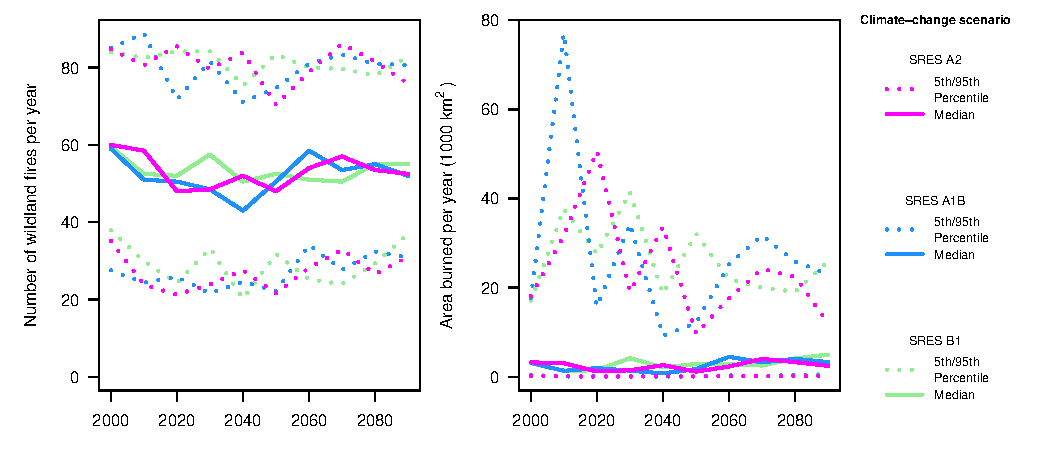
\includegraphics[width=\maxwidth]{figure/fire_change_ts_AK-1} \caption[Alaska]{Alaska\label{fig:fire_change_ts_AK}}
\end{figure}



All five following separate LCC graphs relate to figure 8.3 in the original document.
This uses strictly ALFRESCO output.

\subsection{Arctic}
\begin{figure}[H]
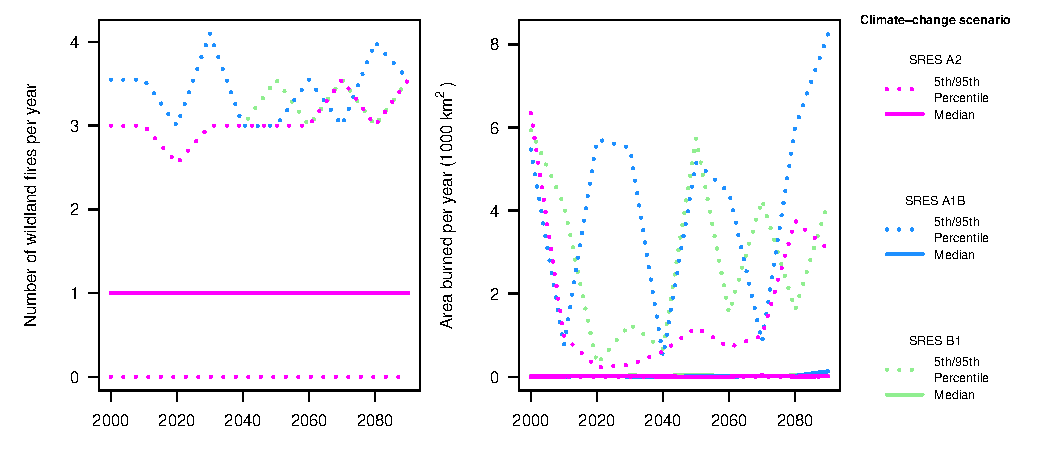
\includegraphics[width=\maxwidth]{figure/fire_change_ts_LCC1-1} \caption[Arctic]{Arctic\label{fig:fire_change_ts_LCC1}}
\end{figure}



\subsection{North Pacific}
\begin{figure}[H]
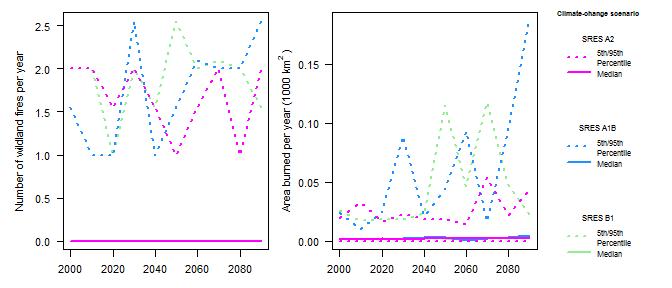
\includegraphics[width=\maxwidth]{figure/fire_change_ts_LCC2-1} \caption[North Pacific]{North Pacific\label{fig:fire_change_ts_LCC2}}
\end{figure}



\subsection{Northwest Interior Forest North}
\begin{figure}[H]
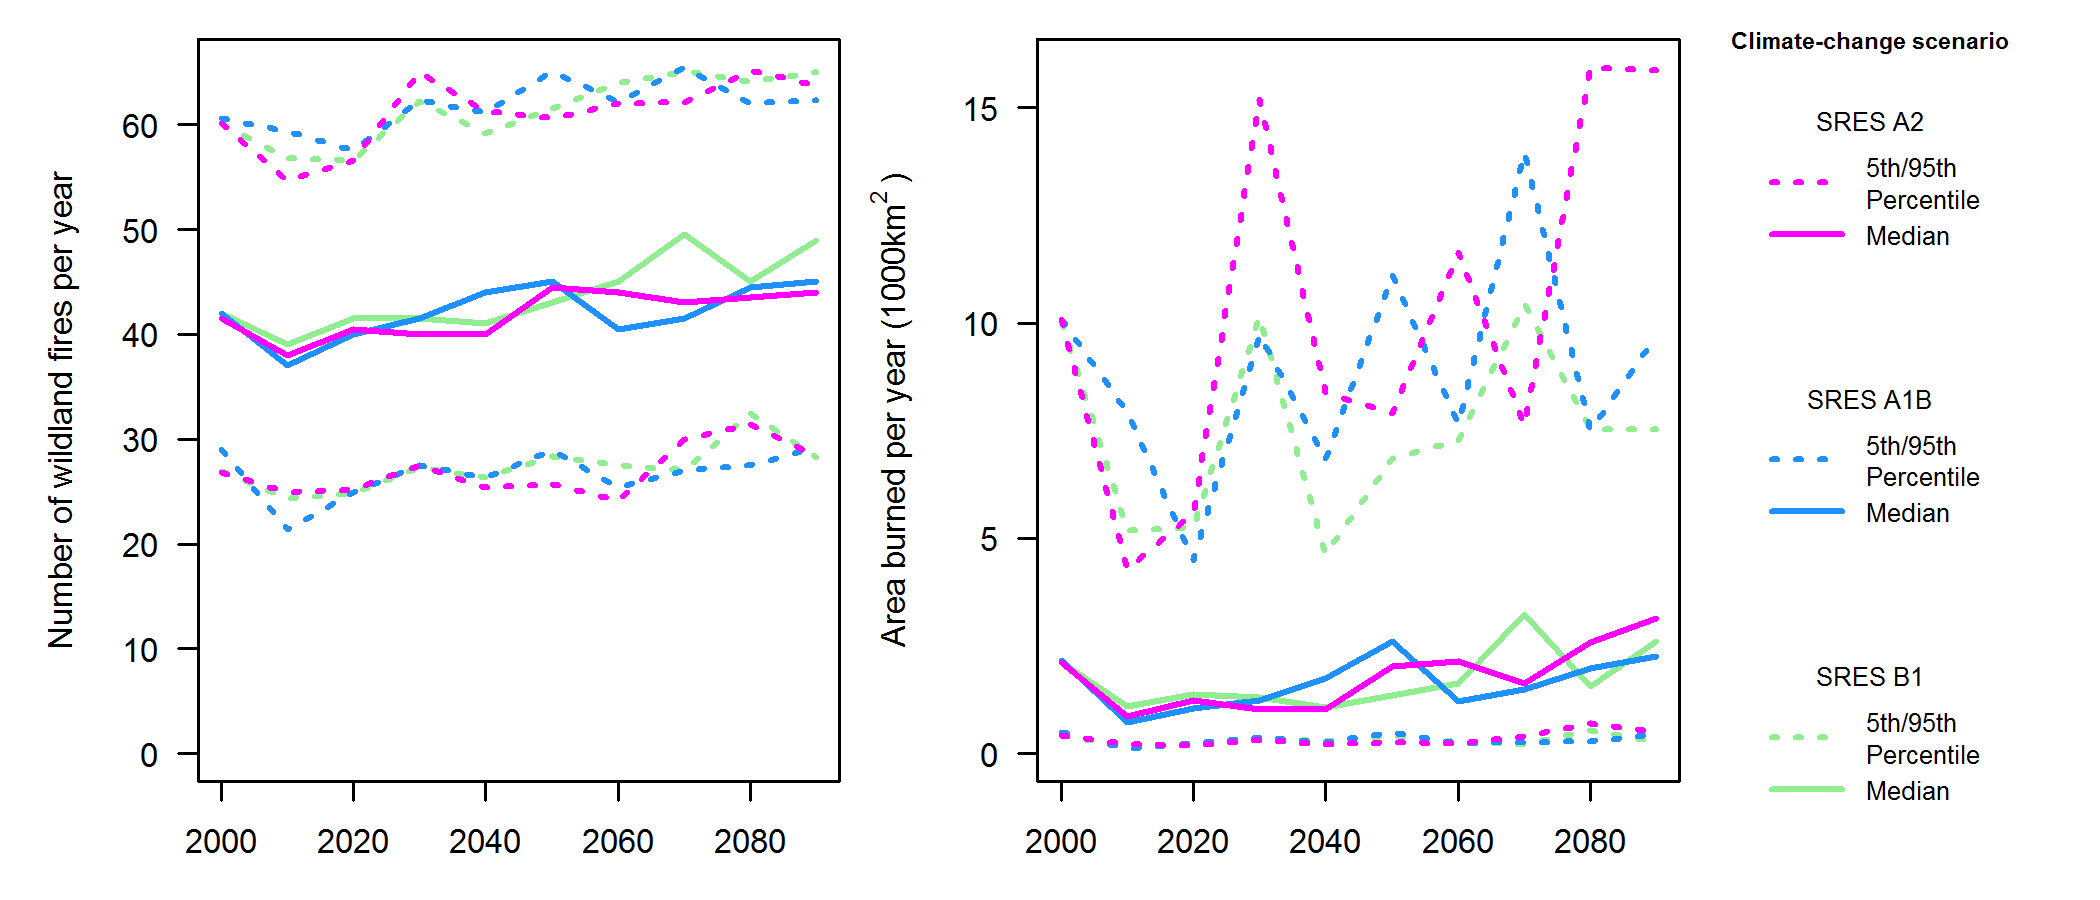
\includegraphics[width=\maxwidth]{figure/fire_change_ts_LCC3-1} \caption[Northwest Interior Forest North]{Northwest Interior Forest North\label{fig:fire_change_ts_LCC3}}
\end{figure}



\subsection{Northwest Interior Forest South}
\begin{figure}[H]
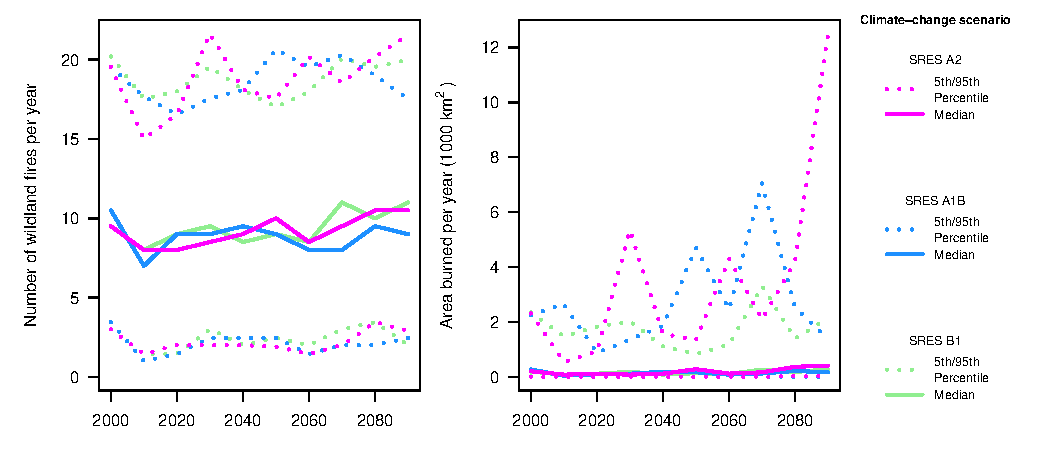
\includegraphics[width=\maxwidth]{figure/fire_change_ts_LCC4-1} \caption[Northwest Interior Forest South]{Northwest Interior Forest South\label{fig:fire_change_ts_LCC4}}
\end{figure}



\subsection{Western Alaska}
\begin{figure}[H]
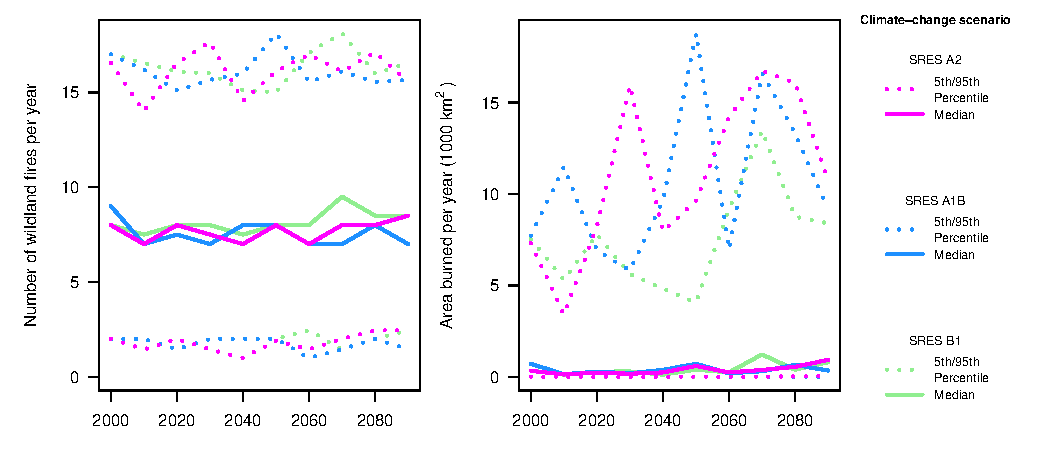
\includegraphics[width=\maxwidth]{figure/fire_change_ts_LCC5-1} \caption[Western Alaska]{Western Alaska\label{fig:fire_change_ts_LCC5}}
\end{figure}



\end{document}
